\section{Calibration}

The calibration of the LTCC detector consisted of matching the gains of the 216 PMTs.
The main reason for this is that the FADC250 thresholds and sampling acquisition parameters are the same for all channels.

\begin{figure*}
	\centering
	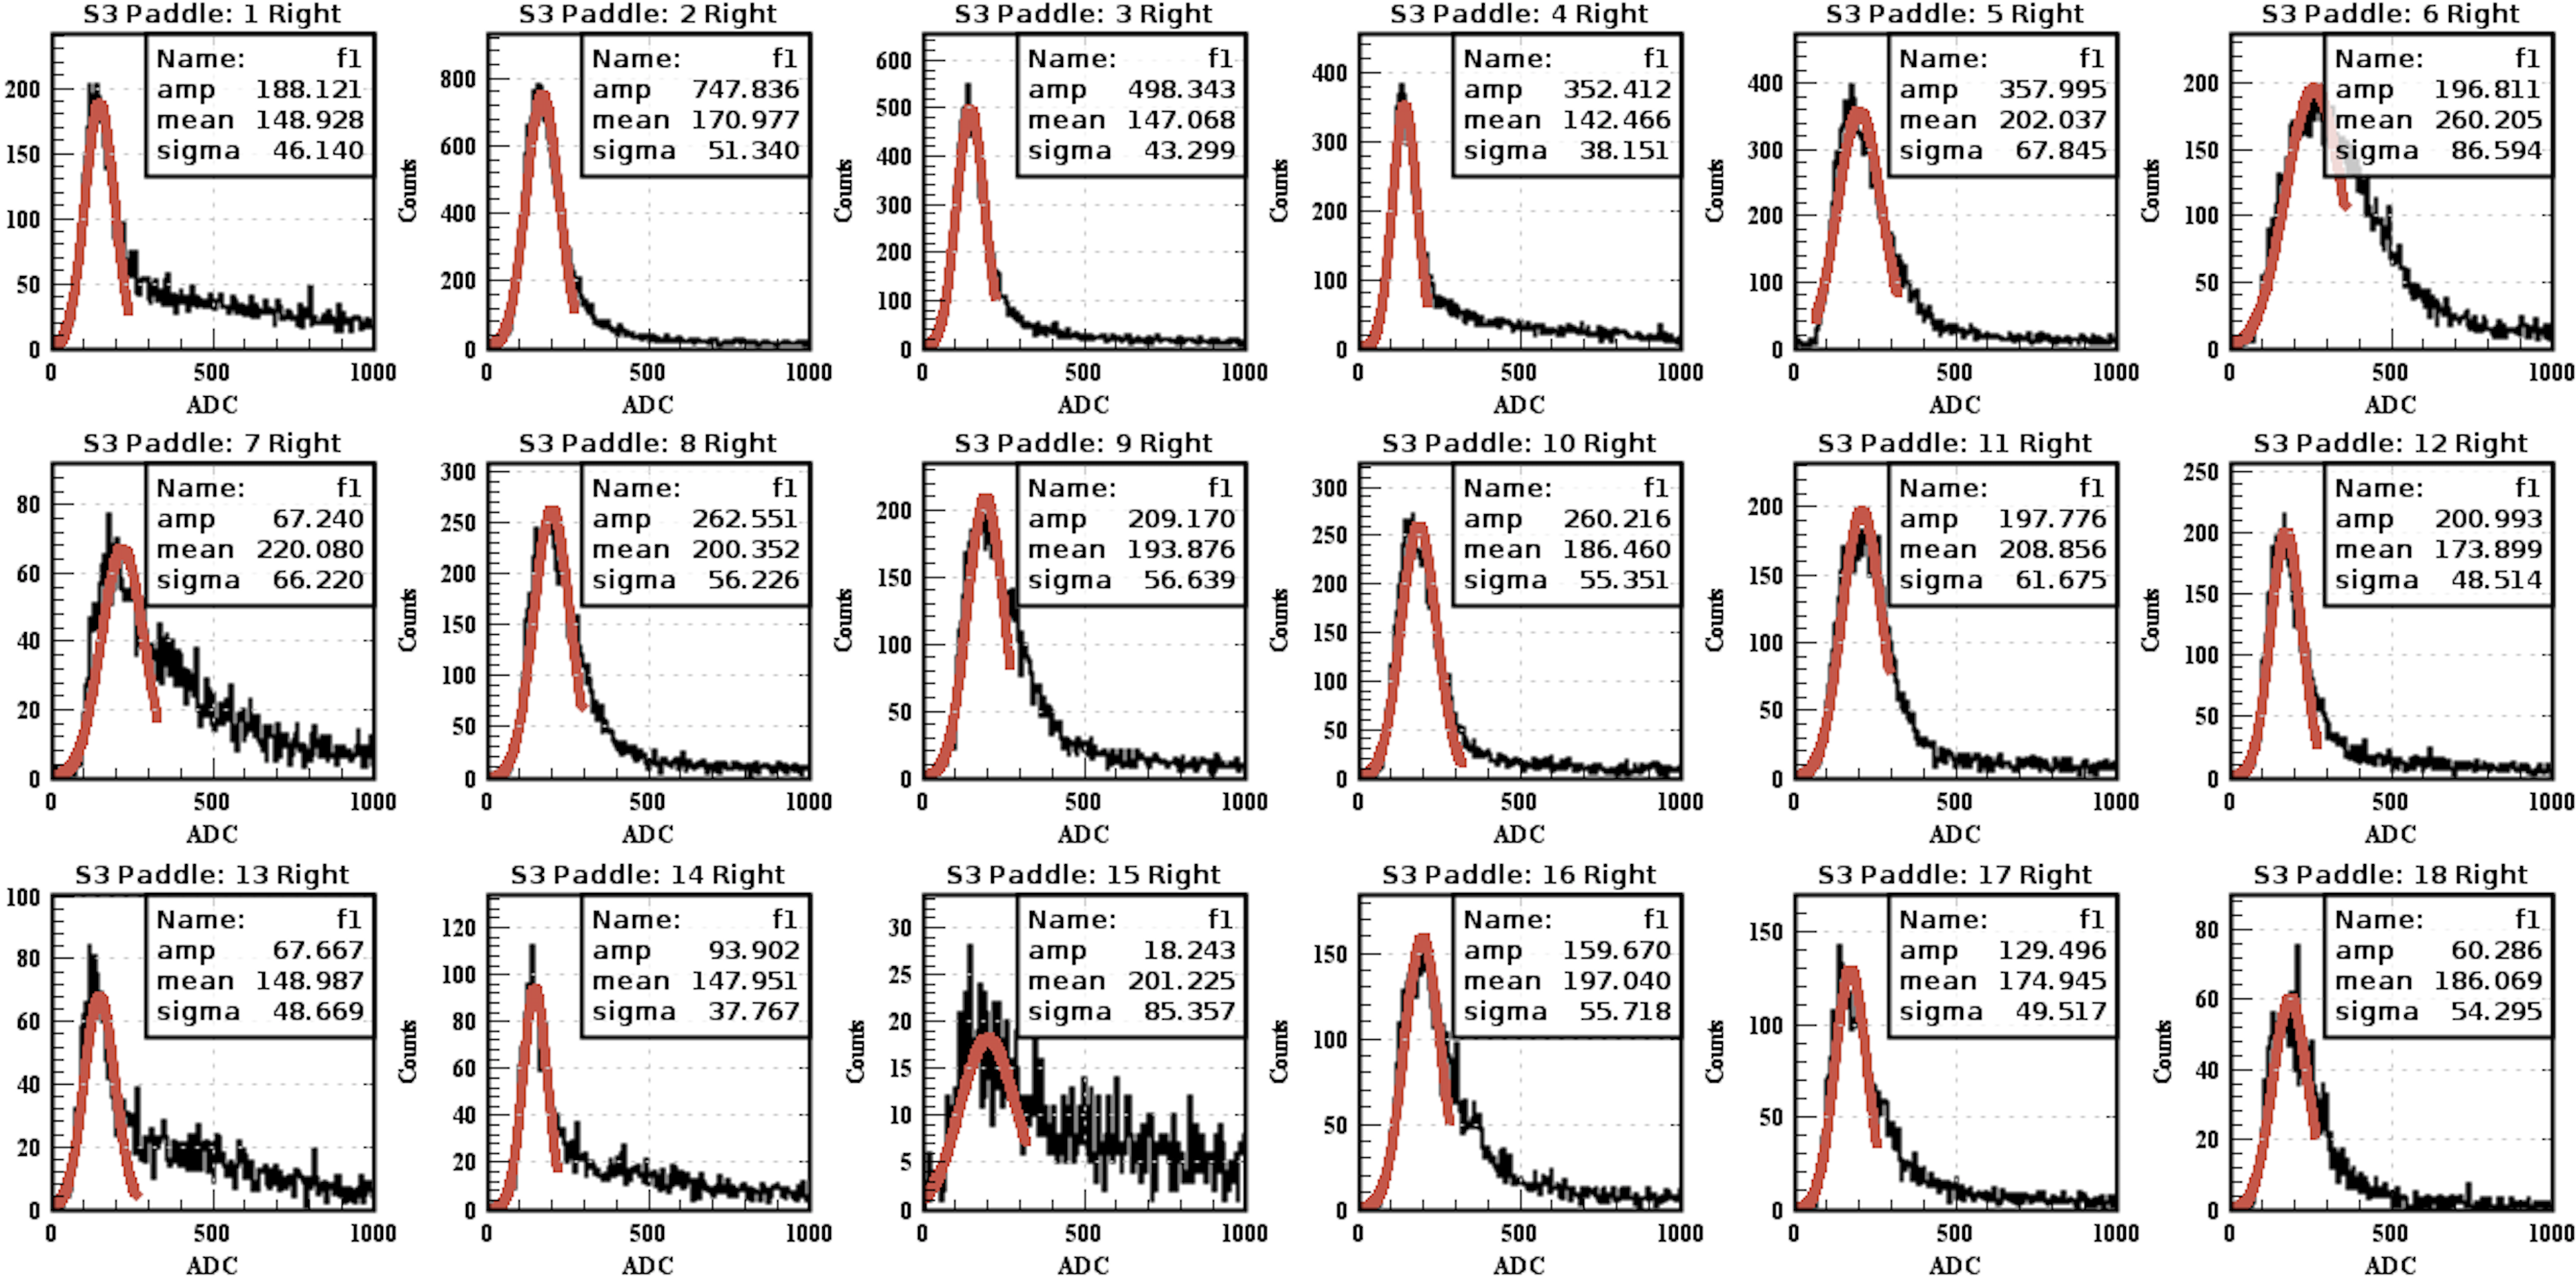
\includegraphics[width=2.1\columnwidth,keepaspectratio]{img/spe.png}
	\caption{The LTCC sector 3 right side ADC spectra. Data is from the first production run in spring 2018.
             The SPE peak positions are fit with a gaussian function and the mean $ADC_M$ parameters are recorded in the calibration database.
             The reconstructed number of photo-electrons for the digitized ADC value is then ADC / $ADC_M$. Some anomalous PMTs can be seen:
             \#6 shows a larger than normal width (too large HV) and \# 15 shows smaller than normal signal to width ratio, probably due to PMT
             hardware problems.}
	\label{fig:speCalibration}
\end{figure*}

This gain calibration was carried out by using data with an electron beam incident on the experiment target.
A random trigger was saved in the data-stream at a rate of 100Hz.
This data subset includes LTCC events with PMT noise above the FADC pedestal, containing the single Photo-electron signal (SPE).

The ADC spectra (see for \F{speCalibration} for typical histograms) were fit to identify the SPE peak positions.
At the beginning of each experiment the PMT high voltages are adjusted to align the peak positions
to a particular ADC value of $ADC_M = 200$. An example of gain matching is shown in \F{gainMatching}.


\begin{figure}[h]
	\centering
	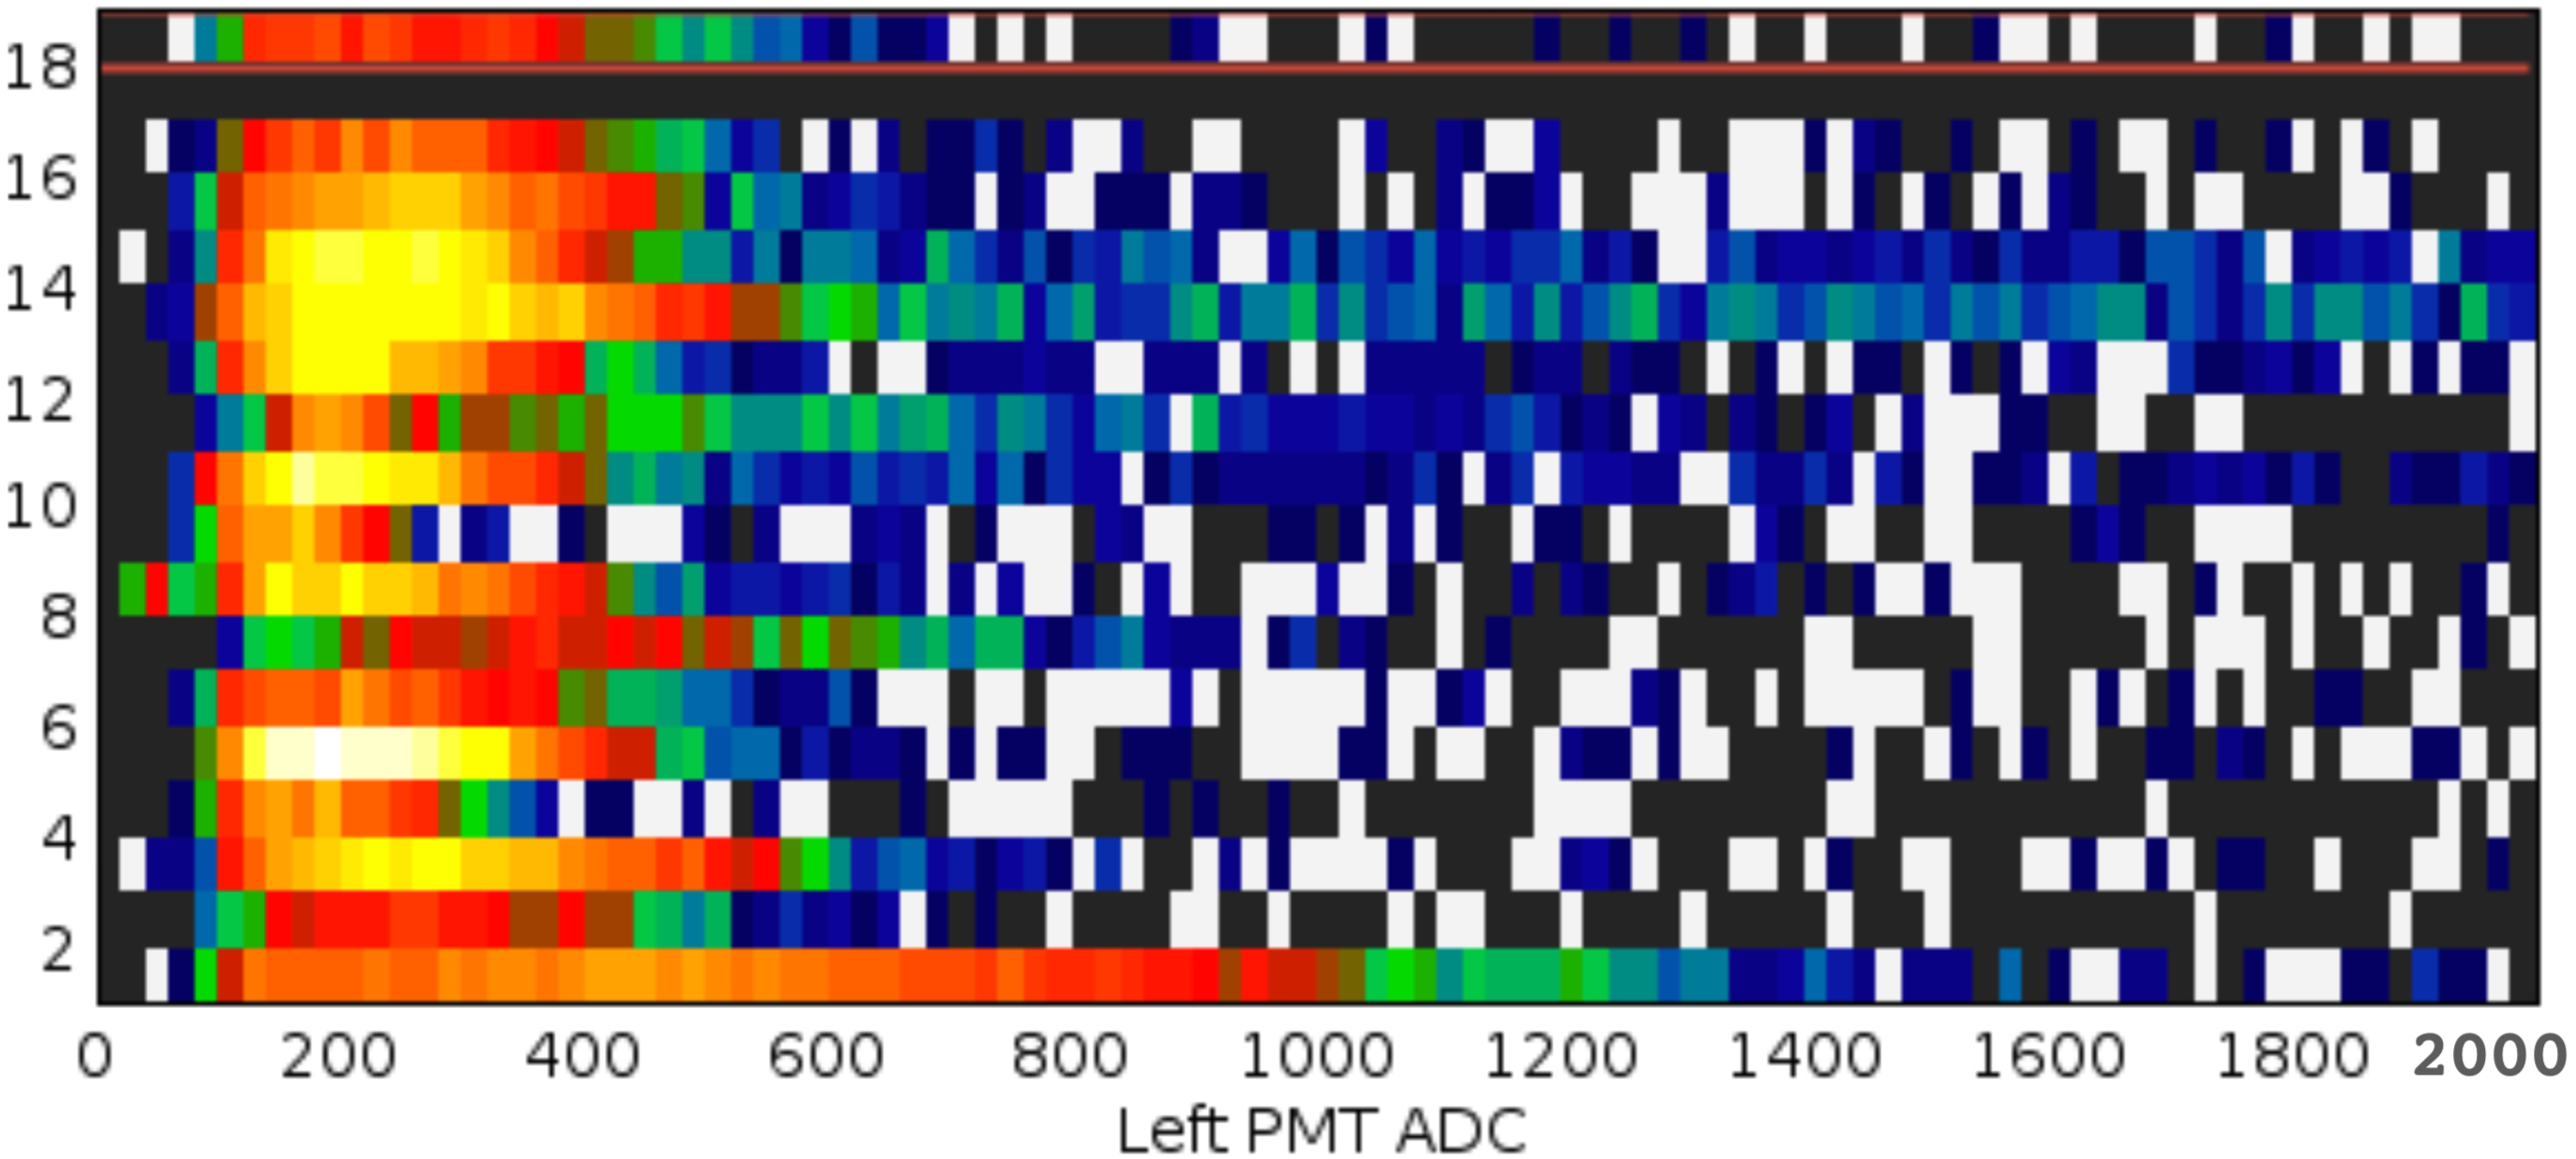
\includegraphics[width=0.99\columnwidth,keepaspectratio]{img/gainMatchingBefore.png}
	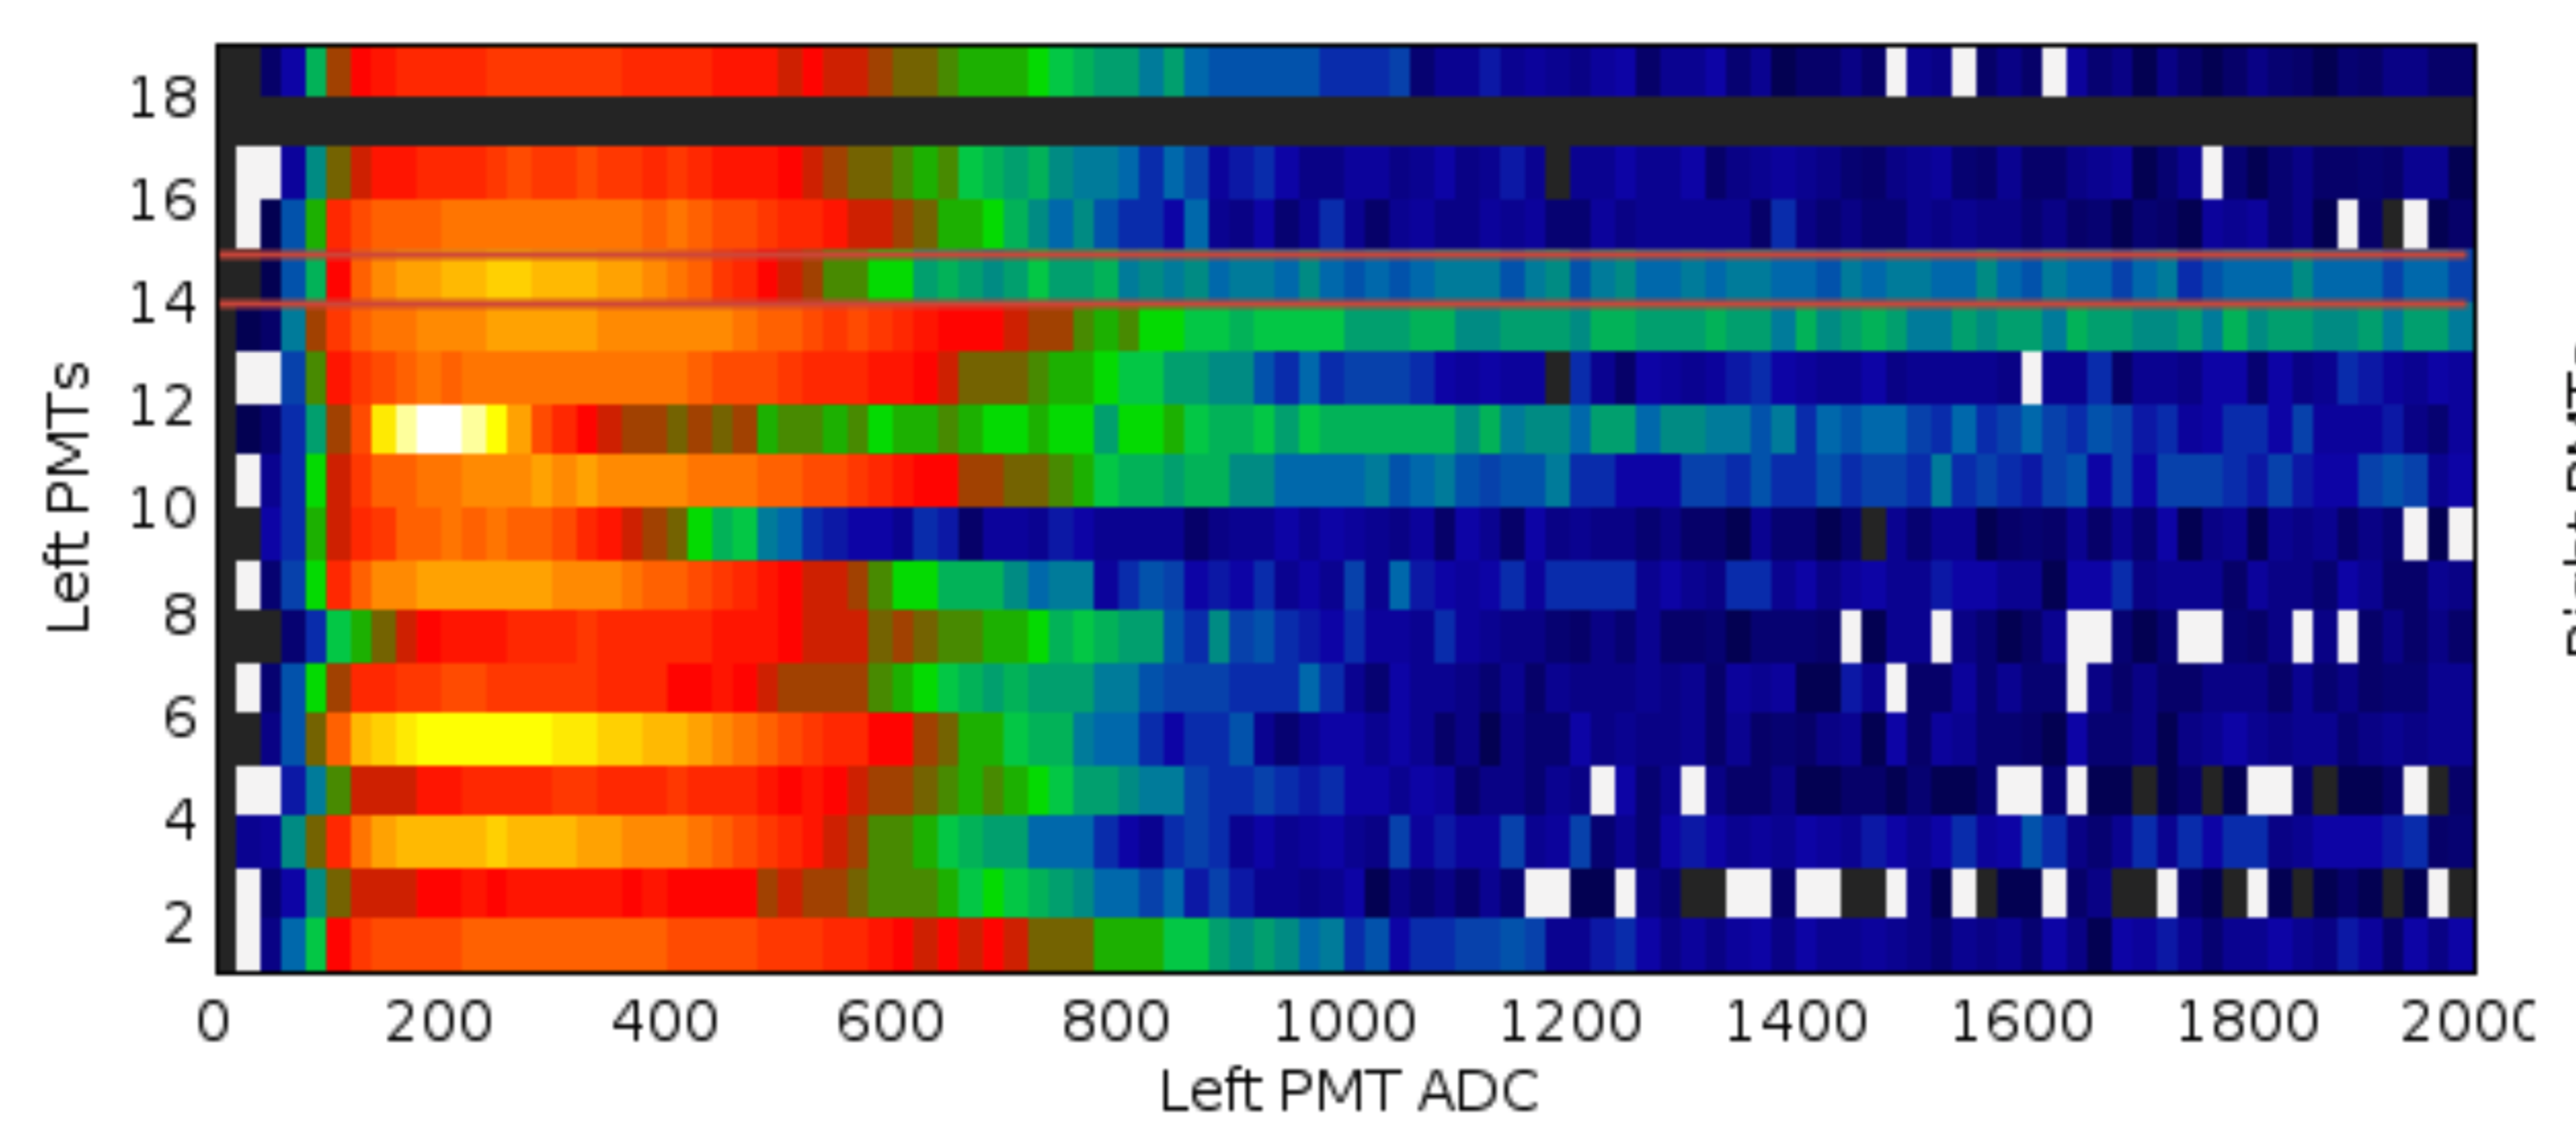
\includegraphics[width=0.99\columnwidth,keepaspectratio]{img/gainMatchingAfter.png}
	\caption{Plot of PMT \# vs ADC for he LTCC sector 3 right side PMTs. Data is from the first production
             run in spring 2018. Top: before gain matching several channels do not show a SPE peak position at  $ADC_M = 200$.
             Bottom: after gain matching the PMT responses are well aligned.}
	\label{fig:gainMatching}
\end{figure}

During analysis of physics events, the reconstructed number of photo-electrons for the digitized ADC value calculated to be ADC / $ADC_M$.

It was found that the gains of several of the phototubes drifted with time, so the calibration procedure was repeated every week to ensure that
the values of $ADC_M$ reflects the latest gains and that these variation do not affect the LTCC response.



